\section{Pianificazione}
 
Con l'obbiettivo di rispettare le scadenze specificate nella sezione \ref{scadenze}, lo sviluppo del progetto è stato suddiviso in sei attività:
 
\begin{itemize}
 
	\item Analisi dei Requisiti di Massima;
 
	\item Analisi dei Requisiti di Dettaglio;
 
	\item Progettazione Architetturale;
 
	\item Progettazione di Dettaglio;
 
	\item Codifica;
 
	\item \gl{Validazione}.
 
\end{itemize}
 
Per ogni attività vene riportato lo specifico \gl{diagramma di Gantt} il quale riporta le milestone di ogni attività e le date di inizio e fine di ciascuna sottoattività.
 

\subsection{Analisi dei Requisiti di Massima}
\textbf{Periodo:} da 2017-11-16 a 2018-01-16\Spazio
Inizia con la scelta del \gl{capitolato} e termina con la consegna dei documenti per la Revisione dei Requisiti.
\begin{itemize}
	\item \textbf{Individuazione degli strumenti:} vengono selezionati gli strumenti per la stesura dei documenti, per il versionamento e per lo sviluppo e la \gl{verifica} del prodotto;
	\item \textbf{Norme di Progetto:} viene redatto il documento \emph{Norme di Progetto v1.0.0} con gli strumenti individuati;  
	\item \textbf{Studio di fattibilità:} viene redatto il documento \emph{Studio di Fattibilità v1.0.0} dove vengono spiegate le motivazioni che ci hanno portato alla scelta del capitolato;
	\item \textbf{Analisi dei Requisiti:} viene iniziata la stesura del documento \emph{Analisi dei Requisiti v1.0.0}, questa sottoattività continuerà fino alla data di consegna;
	\item \textbf{Piano di Progetto:} viene redatto il documento \emph{Piano di Progetto v1.0.0}, in cui vengono analizzati i rischi e vengono pianificate le attività del gruppo; 
	\item \textbf{Piano di Qualifica:} viene redatto il documento \emph{Piano di Qualifica v1.0.0}, in cui vengono descritte le operazioni di verifica e validazione del prodotto;
	\item \textbf{Glossario:} viene redatto il documento \emph{Glossario v1.0.0};
\end{itemize}
\subsubsection{Gantt}
\begin{figure}[H]
	\centering 
	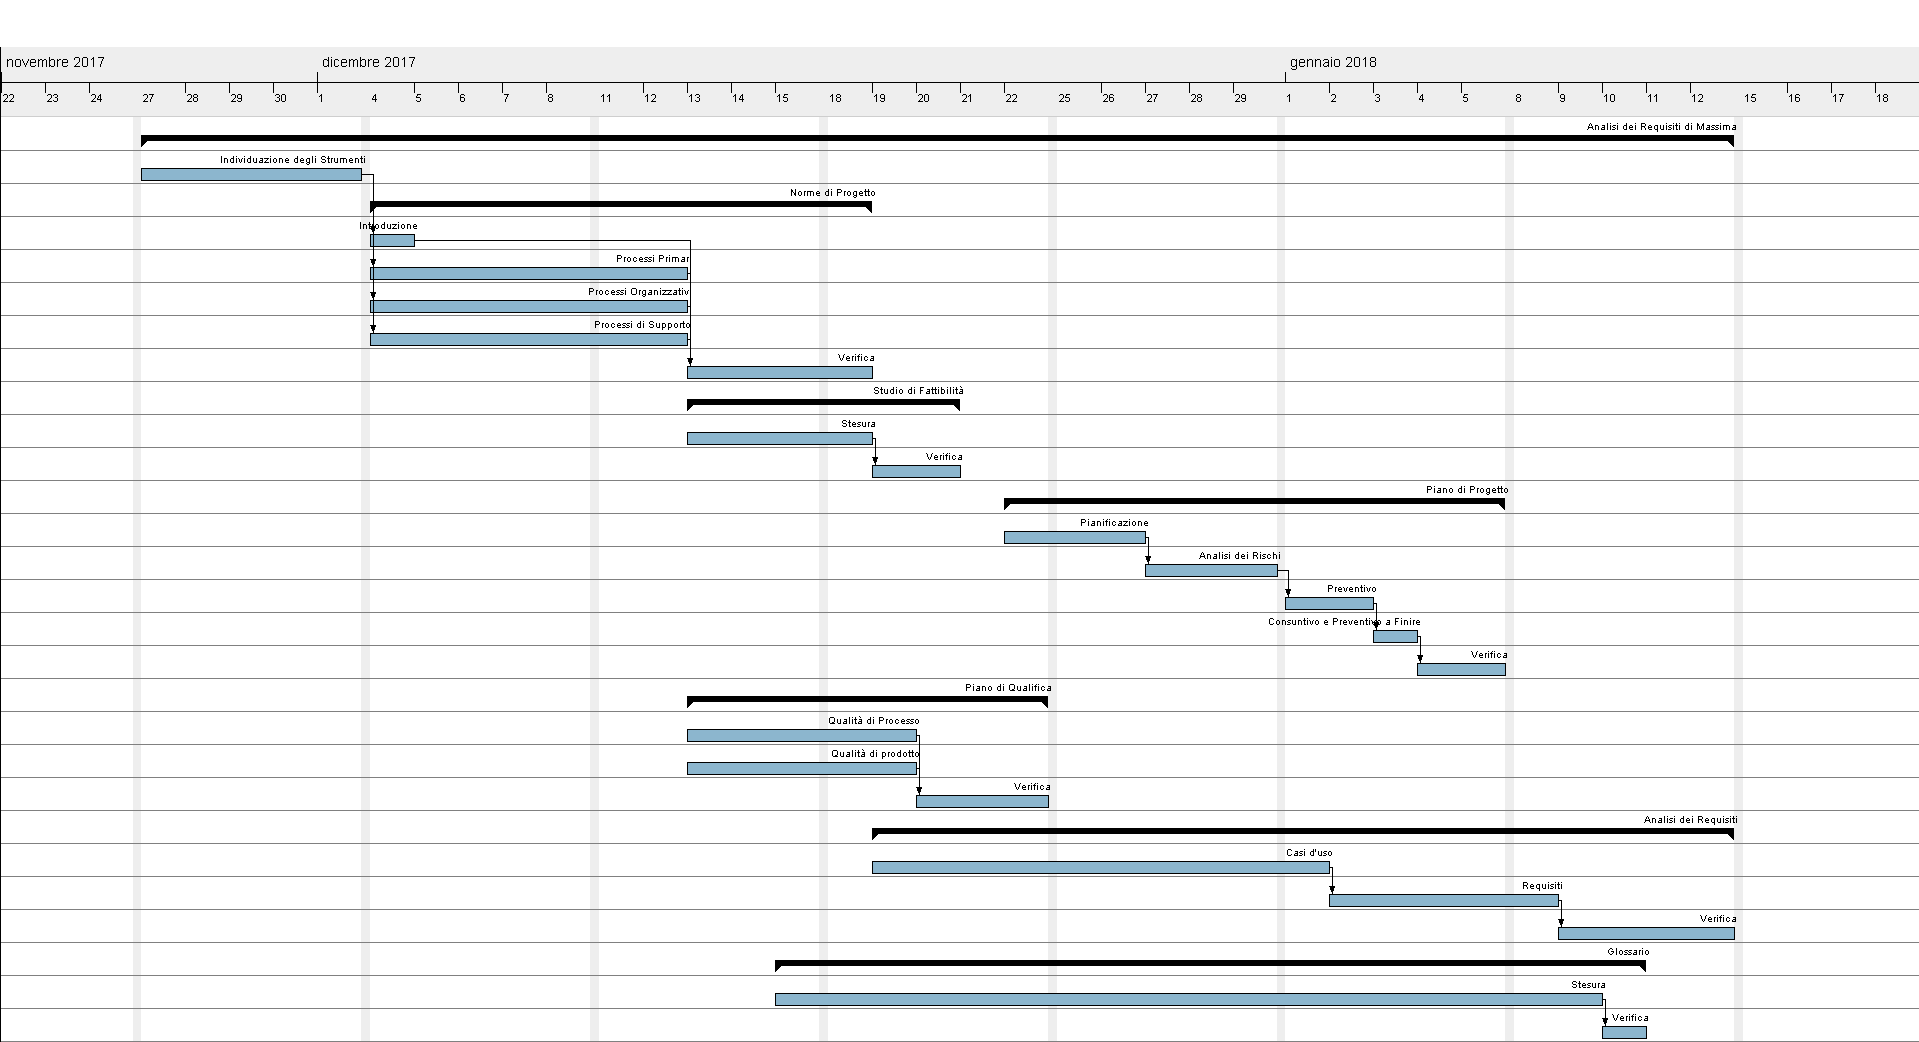
\includegraphics[width=1\textwidth]{images/Analisi-di-Massima.png}
	\caption{Diagramma di Gantt dell'Analisi di Massima}
	\label{graficobello} 
\end{figure}
\subsubsection{Studio Personale}
\textbf{Periodo:} da 2018-01-18 a 2018-02-09 \Spazio
Il gruppo utilizza questo periodo per lo studio personale al fine di sostenere gli appelli d'esame della sessione invernale, inoltre i componenti si impegnano ad approfondire alcune tecnologie utili per lo sviluppo del progetto.
\subsection{Analisi dei Requisiti di Dettaglio}
    \textbf{Periodo:} da 2018-02-09 a 2018-02-21 \Spazio
    Inizia dopo la consegna dei documenti per la Revisione dei Requisiti e termina con l'inizio dell'attività di \emph{Progettazione Architetturale}
    \begin{itemize}
    	\item \textbf{Analisi dei Requisiti:} vengono consolidati i requisiti richiesti dal sistema e viene ampliato il documento \emph{Analisi dei Requisiti v1.0.0};
    	\item \textbf{Incremento e Verifica:} vengono aggiornati e verificati, se necessario, i documenti già redatti. 
    \end{itemize}
\subsubsection{Gantt}
\begin{figure}[H]
	\centering 
	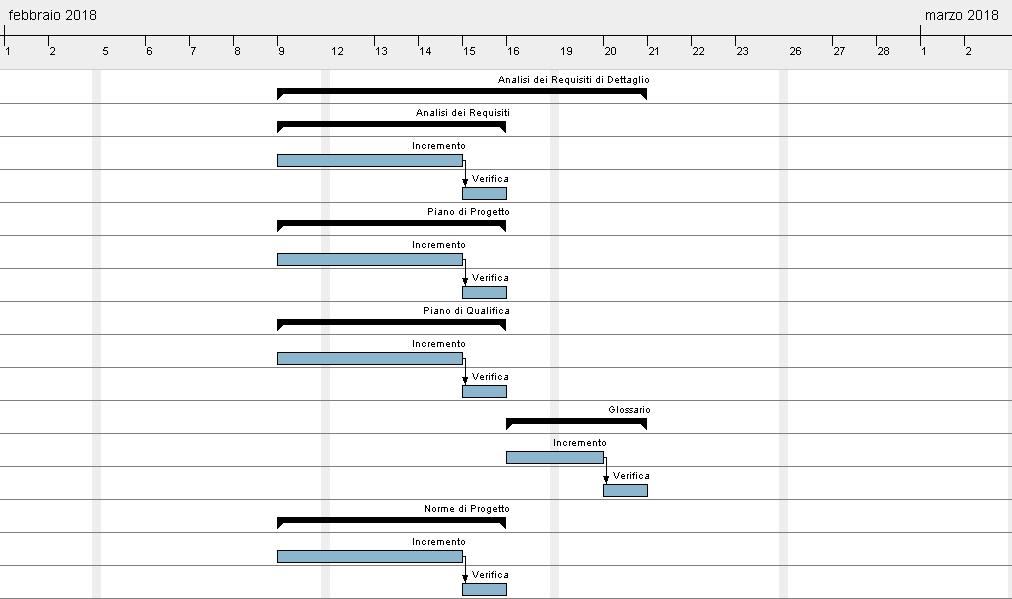
\includegraphics[width=1\textwidth]{images/Analisi-Dettaglio.png}
	\caption{Diagramma di Gantt dell'Analisi di Dettaglio}
	\label{graficobello2} 
\end{figure}
\subsection{Progettazione Architetturale}
    \textbf{Periodo:} da 2018-02-21 a 2018-03-07 \Spazio
    Inizia al termine dell'\emph{Analisi dei Requisiti di Dettaglio} e termina con la consegna del materiale in ingresso alla \emph{Revisione di Progettazione}.
    \begin{itemize}
    	\item \textbf{Technology Baseline:} viene redatto il documento \emph{Technology Baseline } dove vengono presentate le tecnologie selezionate per lo sviluppo del prodotto e ne viene dimostrata l'adeguatezza;
    	\textcolor{red}{fix}
    	\item \textbf{Proof of Concept:} viene sviluppato un Proof of Concept atto a dimostrare l'architettura fondamentale del nostro prodotto e le sue funzionionalità principali;
    	\item \textbf{Incremento e Verifica:} vengono aggiornati e verificati, se necessario, i documenti già redatti.	
    \end{itemize}
\subsubsection{Gantt}
\begin{figure}[H]
	\centering 
	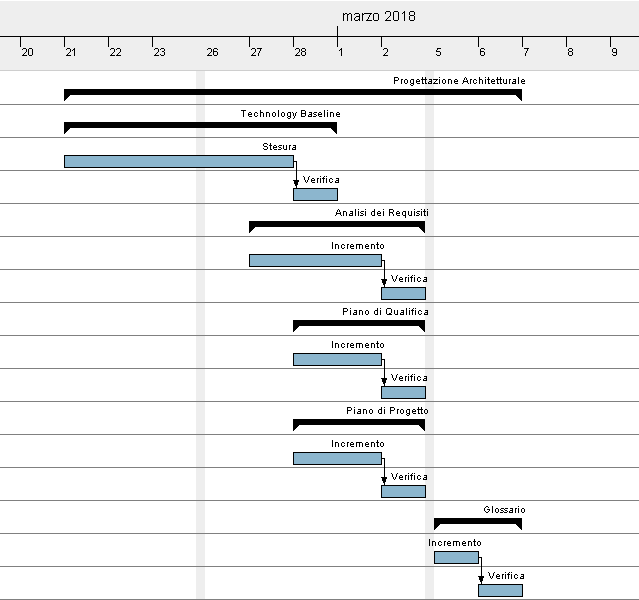
\includegraphics[width=1\textwidth]{images/Progettazione-Architetturale.png}
	\caption{Diagramma di Gantt della Progettazione Architetturale}
	\label{graficobello3} 
\end{figure}
\subsection{Progettazione di Dettaglio}
    \textbf{Periodo:} da 2018-03-20 a 2018-03-27\Spazio
    Inizia dopo la consegna del materiale in ingresso alla \emph{Revisione di Progettazione} e termina con l'inizio dell'attività di codifica.
    \begin{itemize}
    	\item \textbf{Product Baseline:} viene redatto il documento \emph{Product Baseline} il quale presenta l'\gl{architettura} di base del prodotto mostrandone la coerenza con quanto mostrato nel documento \emph{Technology Baseline v1.0.0};
    	\item \textbf{Incremento e Verifica:} vengono aggiornati e verificati,se necessario, i documenti già redatti.
    \end{itemize}
\subsubsection{Gantt}
\begin{figure}[H]
	\centering 
	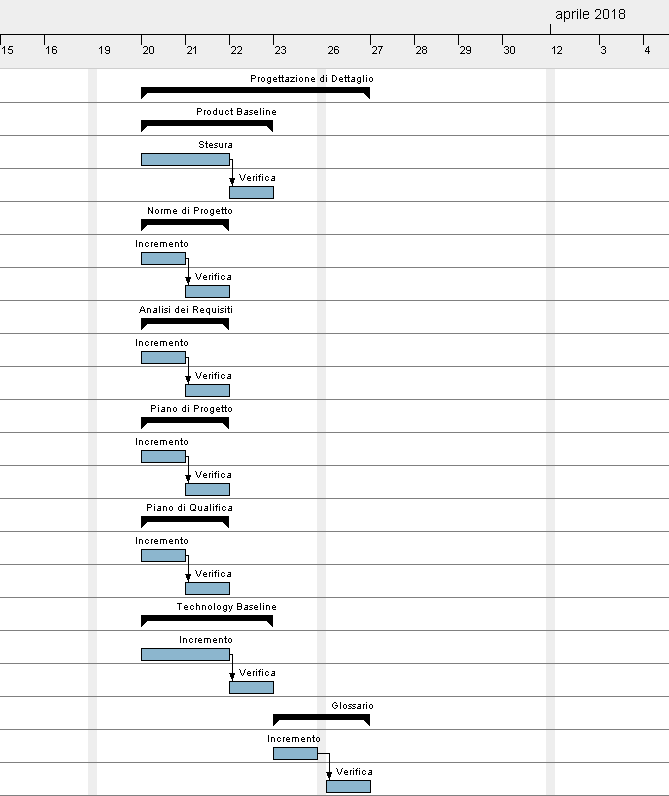
\includegraphics[width=0.9\textwidth]{images/Progettazione-Dettaglio.png}
	\caption{Diagramma di Gantt per la Progettazione di Dettaglio}
	\label{graficobello4} 
\end{figure}
\subsection{Codifica}
    \textbf{Periodo:} da 2018-03-27 a 2018-04-12\Spazio
    Inizia al termine dell'attività di \emph{Progettazione di Dettaglio} e termina con la consegna del materiale in ingresso alla \emph{Revisione di Qualifica}.
    \begin{itemize}
    	\item \textbf{Codifica del Prodotto:} viene sviluppata una versione funzionante del prodotto attraverso due cicli incrementali;
    	\item \textbf{Manuali:} vengono redatti i manuali necessari per aiutare l'utente nell'utilizzo del software;
    	\item \textbf{Incremento e Verifica:} vengono aggiornati e verificati, se necessario, i documenti già redatti.
    \end{itemize}
\subsubsection{Gantt}
\begin{figure}[H]
	\centering 
	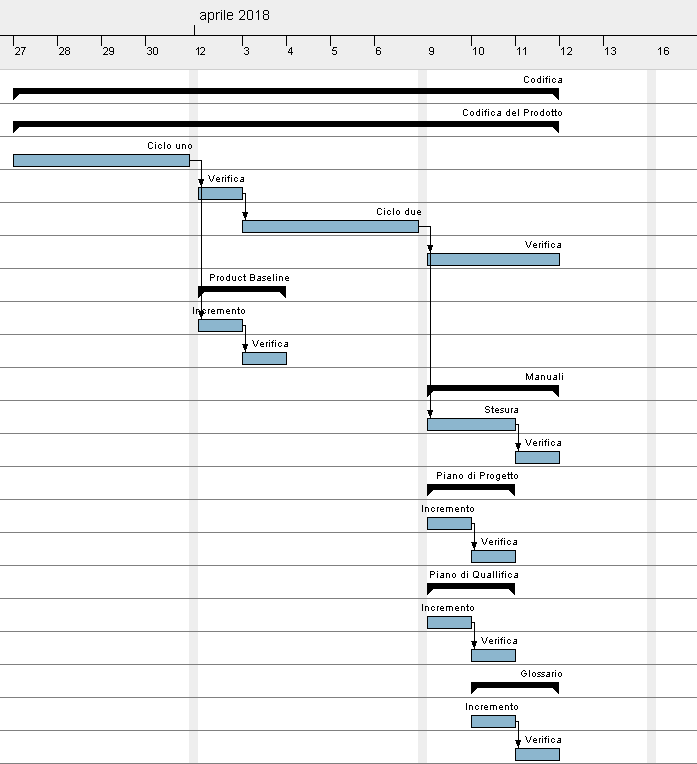
\includegraphics[width=0.7\textwidth]{images/Codifica.png}
	\caption{Diagramma di Gantt per la Codifica}
	\label{graficobello5} 
\end{figure}
\subsection{Validazione}
    \textbf{Periodo:} da 2018-04-23 a 2018-05-04\Spazio
    Inizia dopo la consegna del materiale in ingresso alla \emph{Revisione di Qualifica} e termina con la consegna del materiale in ingresso alla \emph{Revisione di Accettazione}.
    \begin{itemize}
    	\item \textbf{Codifica del prodotto:} vengono raffinate le funzionalità e risolti eventuali problemi;
    	\item \textbf{Incremento e Verifica:} vengono aggiornati e verificati, se necessario, i documenti già redatti; 
    	\item \textbf{Validazione:} viene verificata la conformità del prodotto rispetto a tutti i requisiti indicati nel documento \emph{Analisi dei Requisiti ultima versione};
    	\item \textbf{Collaudo:} viene eseguita e testata ogni funzionalità del prodotto richiesta dal capitolato.
    \end{itemize}
\subsubsection{Gantt}
\begin{figure}[H]
	\centering 
	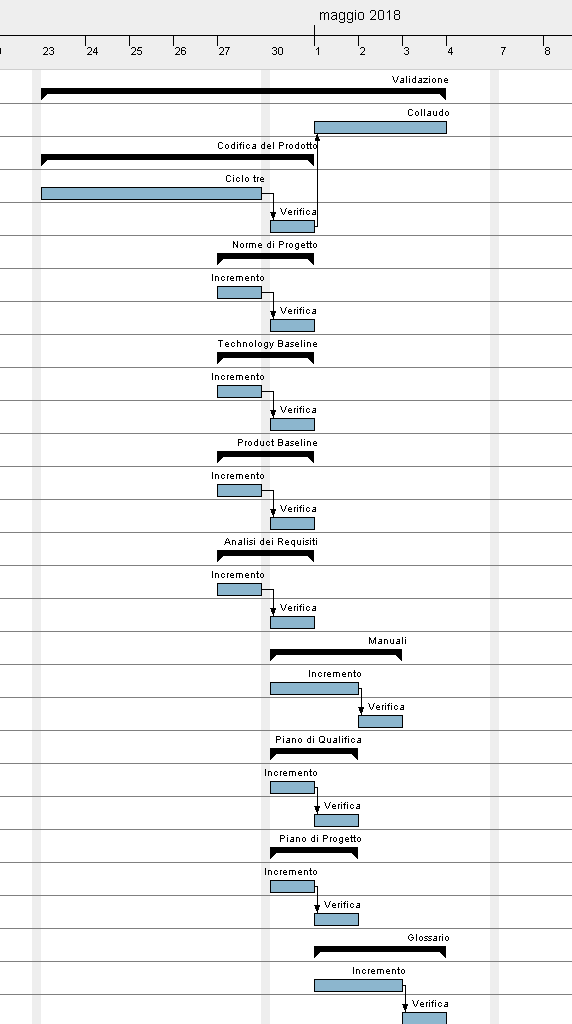
\includegraphics[width=0.7\textwidth]{images/Validazione.png}
	\caption{Diagramma di Gantt per la Validazione}
	\label{graficobello6} 
\end{figure}
